\documentclass[11pt]{article}

\usepackage{minted,xcolor}
\usemintedstyle{monokai}
\definecolor{bg}{HTML}{282828}
\usepackage{xcolor}
\usepackage{graphicx}
\usepackage{titlesec}
\usepackage[hmargin=2cm,vmargin=2.5cm]{geometry}
\usepackage{fancyhdr}
\usepackage{url}

% \definecolor{line3Color}{HTML}{FFD300}
% \definecolor{line10Color}{HTML}{003688}

\setlength\parindent{0cm}
\setlength\headheight{28pt}

% \titleformat{\section}{\normalfont\huge\bfseries}{Part~\thesection:}{6pt}{}[{\titlerule[0.5pt]}]
% \titleformat{\subsection}{\normalfont\Large\bfseries}{Exercise~\thesubsection:}{6pt}{}

\graphicspath{ {./img/} }

% \title{Practical’s instruction – Networks (week 7)}
% \author{CSC3833 - Data Visualization and Visual Analytic}

\begin{document}

\pagestyle{fancy}
\renewcommand{\headrulewidth}{0pt}
\fancyhead[L]{CSC3833 - Data Visualization and Visual Analytic}
\fancyhead[R]{2023 / 2024}

\begin{center}
\vspace*{1cm}
{\textbf {\Huge Practical Week 6}}\\
\vspace*{0.5cm}
{\textbf {\huge Maps}}
\vspace*{1cm}
\end{center}


\section{Display a map}
% -----------------------------------------------------------------------------------------------------

To display a map, you will need some cartography background and additional datasets. To do so, you can rely on two libraries: \textit{vega\_datasets} and \textit{geopandas}.\\
\\
Make sure \textit{geopandas} is installed before loading it.

\begin{minted}[bgcolor=bg, frame=lines, framesep=2mm]{python}
pip install geopandas
\end{minted}

\begin{minted}[bgcolor=bg, frame=lines, framesep=2mm]{python}
import altair as alt
from vega_datasets import data
import geopandas as gpd
\end{minted}

Once the libraries are loaded, you can load the cartography background, selecting only a few variables of interest and display a first map.

\begin{minted}[bgcolor=bg, frame=lines, framesep=2mm]{python}
# Source of the cartography background
url = "https://naciscdn.org/naturalearth/110m/cultural/ne_110m_admin_0_countries.zip"
countries_shape = gpd.read_file(url)  # zipped shapefile
countries_shape = countries_shape[['NAME', 'CONTINENT', 'ISO_A3', 'geometry']]
\end{minted}

\textit{NAME} corresponds to the name of the country, \textit{CONTINENT} to the continent, \textit{ISO\_A3} is a unique identifier, and \textit{geometry} represents the shape and location of each country.\\
\\
You then need to use the function \textit{mark\_geoshape} to display your first map. You can also specify a projection. For this example we are using the orthographic one.

\begin{minted}[bgcolor=bg, frame=lines, framesep=2mm]{python}
alt.Chart(countries_shape).mark_geoshape(
    ).project('orthographic'
    ).properties(width=600, height=400)
\end{minted}

\subsubsection*{Expected result}

\begin{center}
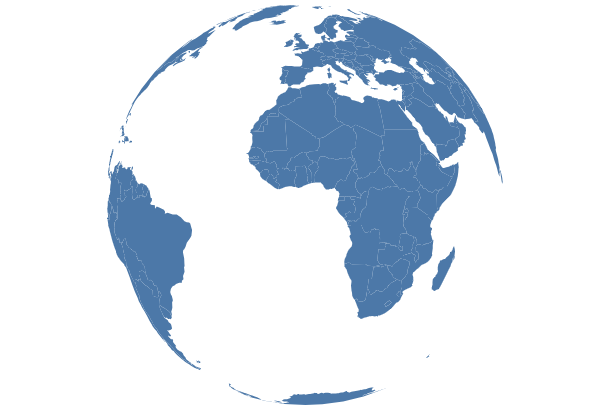
\includegraphics[width=.6\textwidth]{visualization (1).png}
\end{center}

You can decide to add meridians and parallels (graticules) and a sphere background. To do so, start by loading the data for Altair datasets.

\begin{minted}[bgcolor=bg, frame=lines, framesep=2mm]{python}
# Data generators for the background
sphere = alt.sphere()
graticule = alt.graticule()
\end{minted}

Now you need to create your basemap and countries and apply the same projection to them.

\begin{minted}[bgcolor=bg, frame=lines, framesep=2mm]{python}
basemap = (
    alt.layer(
        alt.Chart(sphere).mark_geoshape(fill='white'),
        alt.Chart(graticule).mark_geoshape(stroke='black')
    )
)

countries = (alt.Chart(countries_shape).mark_geoshape())

(basemap + countries).project('orthographic').properties(width=600, height=400)
\end{minted}

\subsubsection*{Expected result}

\begin{center}
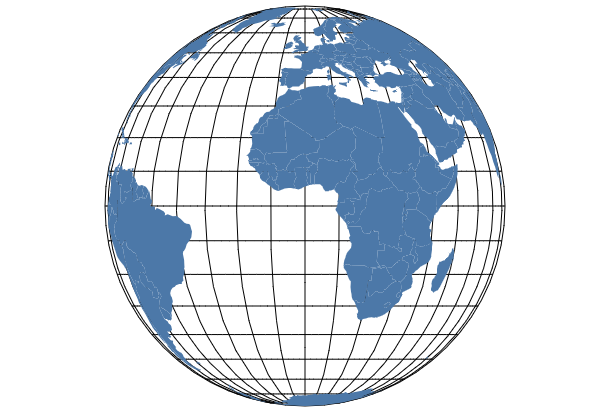
\includegraphics[width=.6\textwidth]{visualization (2).png}
\end{center}

\section{Customize the projection}
% -----------------------------------------------------------------------------------------------------

Altair proposes different projections. Try with \textit{mercator} or \textit{equalEarth}.

\begin{minted}[bgcolor=bg, frame=lines, framesep=2mm]{python}
(basemap + countries).project('equalEarth').properties(width=600, height=400)
\end{minted}

You can even access all of them at once. To do so, create a dropdown menu with all the existing projections and bind it to a parameter.

\begin{minted}[bgcolor=bg, frame=lines, framesep=2mm]{python}
# Dropdown menu of available projections
input_dropdown = alt.binding_select(options=[
    "albers",
    "albersUsa",
    "azimuthalEqualArea",
    "azimuthalEquidistant",
    "conicEqualArea",
    "conicEquidistant",
    "equalEarth",
    "equirectangular",
    "gnomonic",
    "mercator",
    "naturalEarth1",
    "orthographic",
    "stereographic",
    "transverseMercator"
], name='Projection ')

param_projection = alt.param(value="equalEarth", bind=input_dropdown)
\end{minted}

Now add your parameter to the view.

\begin{minted}[bgcolor=bg, frame=lines, framesep=2mm]{python}
((basemap + countries)
    .project(alt.expr(param_projection.name))
    .add_params(param_projection)
    .properties(width=600, height=400)
)
\end{minted}

\subsubsection*{Expected result}

\begin{center}
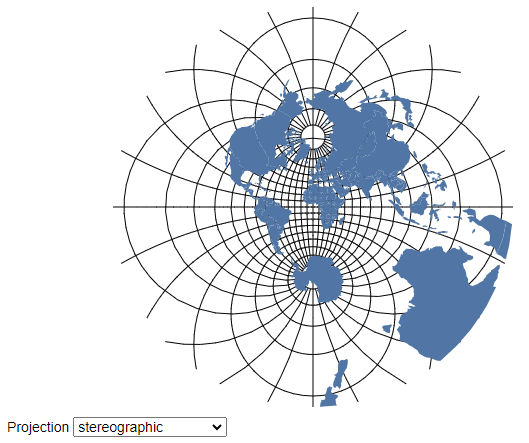
\includegraphics[width=.6\textwidth]{visualization (3).png}
\end{center}

\section{Customize the representation}
% -----------------------------------------------------------------------------------------------------

You can also experiment with the different colours of the view. For instance, try changing the meridians' colour to \textit{LightGray} and the countries to \textit{Coral}.

\begin{minted}[bgcolor=bg, frame=lines, framesep=2mm]{python}
basemap = alt.layer(
        alt.Chart(sphere).mark_geoshape(fill='white'),
        alt.Chart(graticule).mark_geoshape(stroke='LightGray', strokeWidth=0.5)
    )
countries = alt.Chart(countries_shape).mark_geoshape(fill='Coral', stroke='white')

(basemap + countries).project('equalEarth').properties(width=600, height=400)
\end{minted}

The colours used are the standard HTML colours. You can find a detailed table here:
\url{https://en.wikipedia.org/wiki/Web_colours}

\subsubsection*{Expected result}

\begin{center}
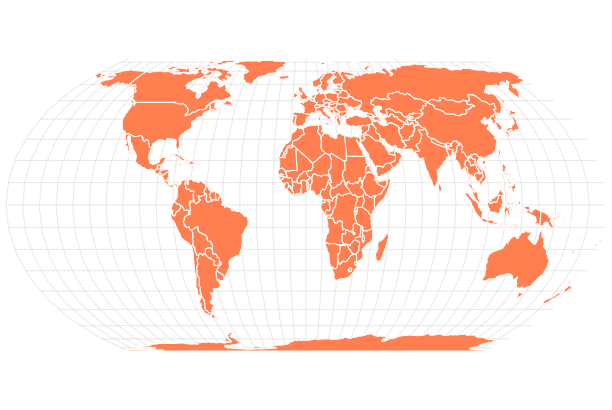
\includegraphics[width=.6\textwidth]{visualization (4).png}
\end{center}

\section{Choropleth}
% -----------------------------------------------------------------------------------------------------

Now that you've mastered the map representation, let's try to encode some data.\\
\\
Start by importing the \textit{Pandas} library and loading the data file used in this practical.

\begin{minted}[bgcolor=bg, frame=lines, framesep=2mm]{python}
import pandas as pd

wasteData = pd.read_csv('goal11.waste.csv')
\end{minted}

The data file contains the amount of waste per capita for each country. Countries are identified by their ISO code, which is also available in the cartography background.\\
\\
The first step is to associate these two files and encode the variable \textit{wastepercap} using color. To do this, we rely on the \textit{transform\_lookup} function. The Lookup transform extends a primary data source by looking up values from another data source; it is similar to a one-sided join.

\begin{minted}[bgcolor=bg, frame=lines, framesep=2mm]{python}
choropleth = (
    alt.Chart(countries_shape)
    .mark_geoshape()
    .transform_lookup(
        lookup='ISO_A3',
        from_=alt.LookupData(data=wasteData, key='iso3c', fields=['wastepercap'])
    )
    .encode(color='wastepercap:Q')
)

(basemap + choropleth).project("equalEarth").properties(width=600, height=400)
\end{minted}

The field \textit{wasteparcap} is now associated with the \textit{country\_shape} dataset.

\subsubsection*{Expected result}

\begin{center}
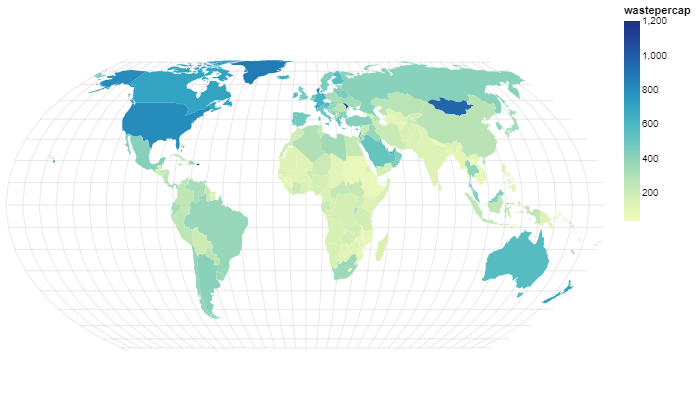
\includegraphics[width=.6\textwidth]{visualization (5).png}
\end{center}

\section{Bubble Map}
% -----------------------------------------------------------------------------------------------------

We now want to represent our data with a point at the center of each country. To do so, we need to transform the \textit{countries\_shape} dataset into \textit{countries\_centroid}, to be able to access the center of each country.

\begin{minted}[bgcolor=bg, frame=lines, framesep=2mm]{python}
countries_centroid = gpd.GeoDataFrame(
    data=countries_shape.copy(),
    geometry=countries_shape.geometry.to_crs(epsg=3857).centroid.to_crs(epsg=4326)
)

countries_centroid["lon"] = countries_centroid.geometry.x
countries_centroid["lat"] = countries_centroid.geometry.y
\end{minted}

You can now represent your basemap and country background, and add circles based on the data using \textit{mark\_circle}. Let's display the size of the circle based on the population size. To do so, add the \textit{pop} field to the \textit{transform\_lookup} function and to the side encoding parameter.

\begin{minted}[bgcolor=bg, frame=lines, framesep=2mm]{python}
countries = (alt.Chart(countries_shape).mark_geoshape(fill='Silver', stroke='white'))

bubbles = (
    alt.Chart(countries_centroid)
    .mark_circle()
    .transform_lookup(
        lookup='ISO_A3',
        from_=alt.LookupData(data=wasteData, key='iso3c', fields=['wastepercap', 'pop'])
    )
    .encode(
        longitude="lon:Q",
        latitude="lat:Q",
        color='wastepercap:Q',
        size='pop:Q'
    )
)

(basemap + countries + bubbles).project("equalEarth").properties(width=600, height=400)
\end{minted}

\subsubsection*{Expected result}

\begin{center}
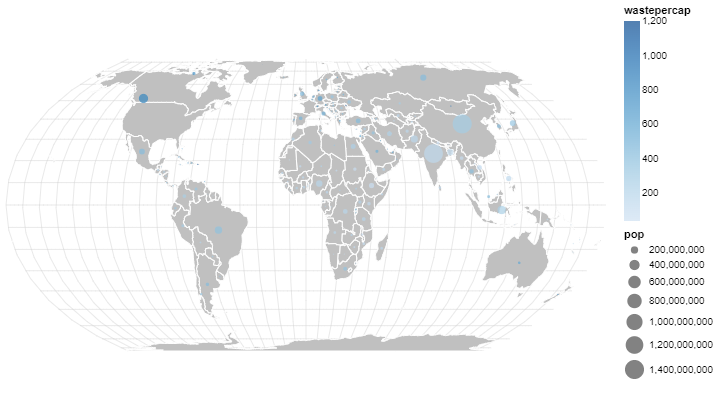
\includegraphics[width=.6\textwidth]{visualization (6).png}
\end{center}

\section{Colour Scale}
% -----------------------------------------------------------------------------------------------------

Now we want to change the colour scale. We first need to create a specific colour scale and add it to the map.

\begin{minted}[bgcolor=bg, frame=lines, framesep=2mm]{python}
colorScale = alt.Color(
    "wastepercap:Q",
    scale = alt.Scale(scheme="inferno"),
    legend = alt.Legend(direction="horizontal", orient="bottom")
)

bubbles = (
    alt.Chart(countries_centroid)
    .mark_circle()
    .transform_lookup(
        lookup='ISO_A3',
        from_=alt.LookupData(data=wasteData, key='iso3c', fields=['wastepercap', 'pop'])
    )
    .encode(
        longitude="lon:Q",
        latitude="lat:Q",
        color=colorScale,
        size='pop:Q'
    )
)
\end{minted}

The parameter \textit{inferno} refers to the colour scheme. Please have a look at the following link to experiment different colour schemes: \url{https://vega.github.io/vega/docs/schemes/}.\\
\\
The colour is currently applied linearly. Try other types or scales such as \textit{quantile} or \textit{quantize}.

\begin{minted}[bgcolor=bg, frame=lines, framesep=2mm]{python}
colorScale = alt.Color(
    "wastepercap:Q",
    scale = alt.Scale(scheme="inferno", type='quantile')
)
\end{minted}

\subsubsection*{Expected result}

\begin{center}
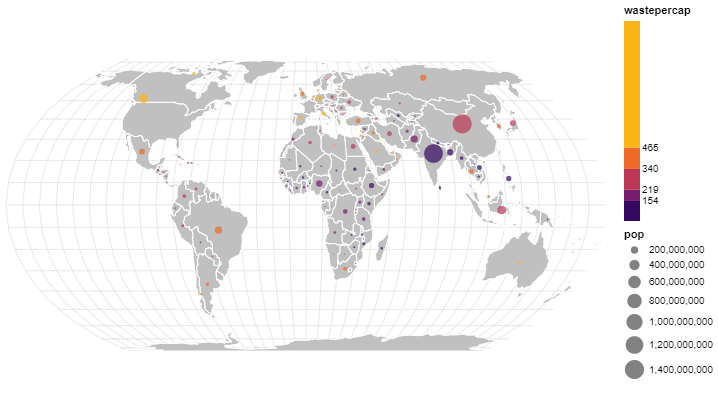
\includegraphics[width=.6\textwidth]{visualization (7).png}
\end{center}

\section{Interaction}
% -----------------------------------------------------------------------------------------------------

\subsection*{Part1}

Like any other chart, a map can be interactive. Try to rely on what you've learned so far, including the previous practical, to select data according to their continent.

\subsubsection*{Expected result}

\begin{center}
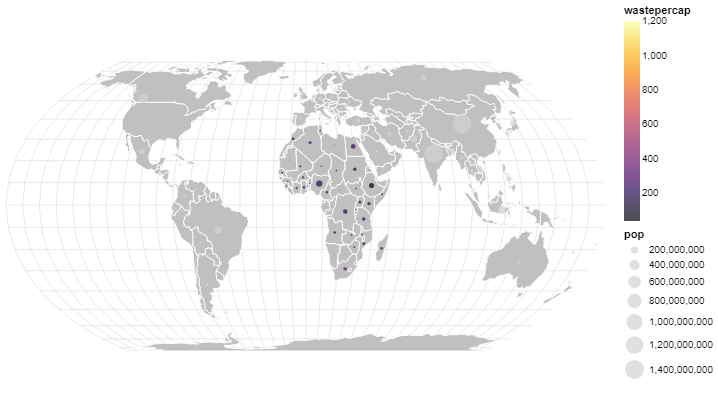
\includegraphics[width=.6\textwidth]{visualization (8).png}
\end{center}

The code solving this question is 'hidden' at the bottom of this document. Try to find the solution yourself first.


\subsection*{Part2}

Often, a map does not come alone but is used in combination with another chart. We will now learn how to link a map with another chart, here a bar chart.\\
\\
First, define a pointer selection for each country independently.

\begin{minted}[bgcolor=bg, frame=lines, framesep=2mm]{python}
# Define a pointer selection
click_countries = alt.selection_point(fields=["NAME"])
\end{minted}

Let's use the choropleth map again, but you can also implement the interaction on the bubble map if you prefer. We want the country to appear more opaque when selected. To do so, apply a condition based on the selection to the opacity of the encoding. Don't forget to add the pointer selection as a parameter.

\begin{minted}[bgcolor=bg, frame=lines, framesep=2mm]{python}
choropleth = (
    alt.Chart(countries_shape)
    .mark_geoshape()
    .transform_lookup(
        lookup='ISO_A3',
        from_=alt.LookupData(data=wasteData, key='iso3c', fields=['wastepercap'])
    )
    .encode(
        color="wastepercap:Q",
        opacity=alt.condition(click_countries, alt.value(1), alt.value(0.2))
    )
    .add_params(click_countries)
)
\end{minted}

Now, let's do the same for the bar chart.

\begin{minted}[bgcolor=bg, frame=lines, framesep=2mm]{python}
bars = (
    alt.Chart(countries_shape)
    .mark_bar()
    .transform_lookup(
        lookup='ISO_A3',
        from_=alt.LookupData(data=wasteData, key='iso3c', fields=['wastepercap'])
    )
    .encode(
        x=alt.X("NAME:N").sort("-y"),
        y="wastepercap:Q",
        opacity=alt.condition(click_countries, alt.value(1), alt.value(0.2)),
        color=colorScale,
    )
    .add_params(click_countries)
)
\end{minted}

Finally, display them next to each other by using the connector \textit{\&}.

\begin{minted}[bgcolor=bg, frame=lines, framesep=2mm]{python}
((basemap + choropleth).project("equalEarth").properties(width=600, height=400) & bars)
\end{minted}

\subsubsection*{Expected result}

\begin{center}
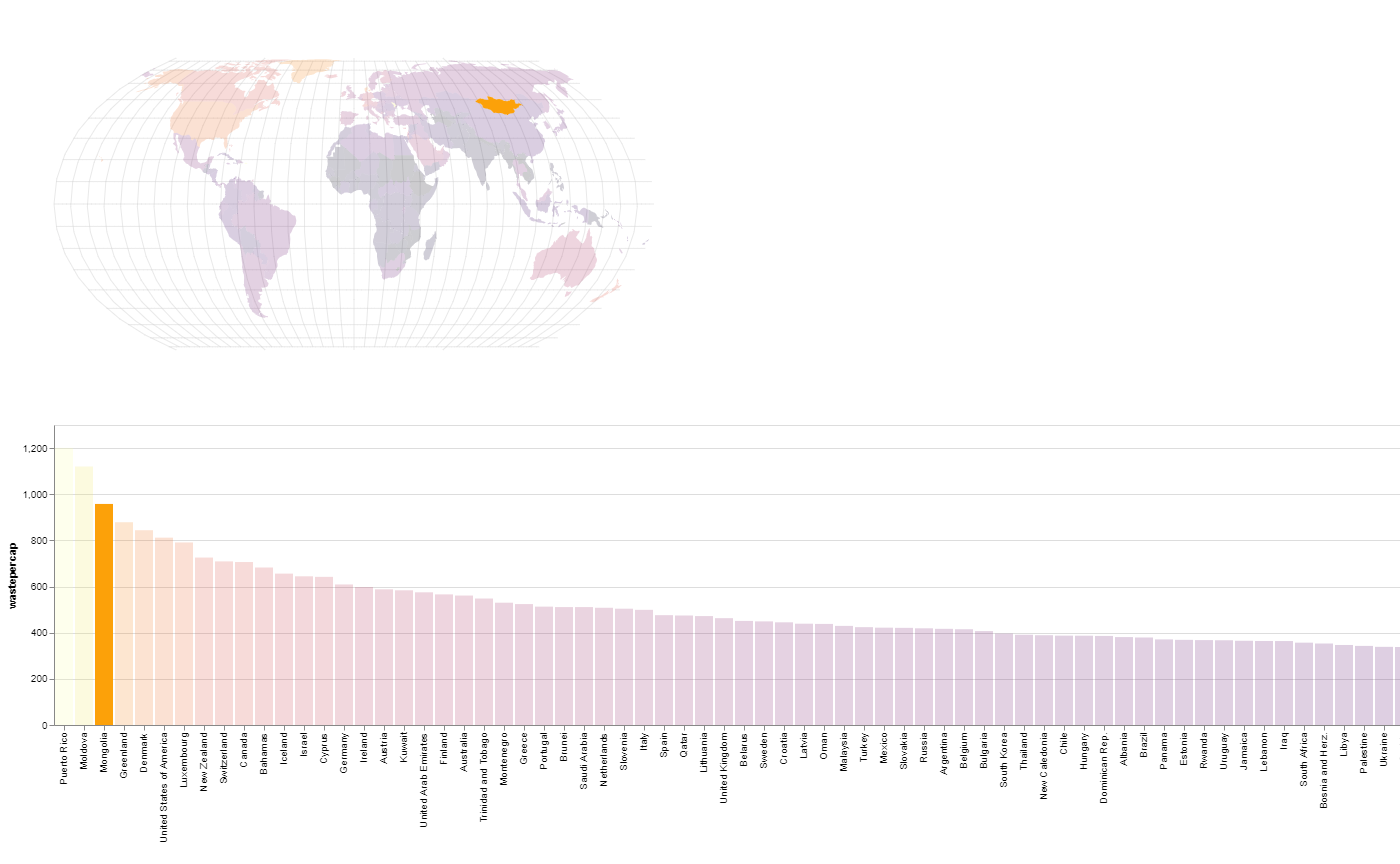
\includegraphics[width=.6\textwidth]{visualization (9).png}
\end{center}

\subsection*{Solution for Part 1}

\begin{itemize}
    \item Create a pointer selection based on the \textit{CONTINENT} variable.
    \item Create a condition based on the selection and display a grey value if the selection is false.
    \item Finally, don't forget to add the pointer selection as a parameter.
\end{itemize}


\begin{minted}[bgcolor=bg, frame=lines, framesep=2mm]{python}
select = alt.selection_point(fields=['CONTINENT'])

bubbles = (
    alt.Chart(countries_centroid)
    .mark_circle()
    .transform_lookup(
        lookup='ISO_A3',
        from_=alt.LookupData(data=wasteData, key='iso3c', fields=['wastepercap', 'pop'])
    )
    .encode(
        longitude="lon:Q",
        latitude="lat:Q",
        color=alt.condition(select, colorScale, alt.value('lightgray')),
        size='pop:Q'
        )
    .add_params(select)
)
\end{minted}


\end{document}